Las herramientas LAT (Lazy Admin Tools en inglés) son una serie de scripts diseñados para automatizar ciertas tareas de administración en SME server. En este momento las herramientas disponibles son:\\

\begin{longtable}{ c | l }
  \textbf{Comando} & \textbf{Descripción} \\\hline
  lat-users & Añadir/borrar usuarios (y sus directorios)\\
  lat-groups & Añadir/borrar grupos\\
  lat-pseudonyms & Añadir/borrar pseudónimos de email para usuarios indivuduales\\
  lat-ibays & Añadir/borrar ibays (y sus directorios)\\
  lat-quota & Determinar la cuota de uso de disco para usuarios individuales\\
  lat-procmail & Activar o desactivar procmail (herramienta de filtrado de email) \\
  & para usuarios individuales\\
  lat-hosts & Añadir o quitar nombres de hosts\\
  lat-domains & Crear dominios virtuales\\
  lat-pptp & Activar o desactivar acceso pptp para usuarios individuales\\
  lat-dump & Crear archivos de input para las herramientas anteriores\\
  lat-shadow & Transferir una contraseña encriptada desde un servidor SME a otro\\
\end{longtable}

Cada una de ellas tiene su entrada correspondiente en el manual. A continuación instalaremos las herramientas LAT y como ejemplo de su utilización usaremos lat-users para crear varios usuarios.

\section{Instalación}

Las herramientas LAT se encuentran en el repositorio 'smecontribs'. Para instalarlas junto a los paquetes necesarios usaremos el siguiente comando:

\begin{lstlisting}
yum install --enablerepo=smecontribs smeserver-lazy_admin_tools smeserver-userpanel smeserver-mailsorting
\end{lstlisting}

Tras instalarlo, nos advierte de que debemos reiniciar:

\begin{lstlisting}
signal-event post-upgrade; signal-event reboot
\end{lstlisting}

\section{lat-users}
lat-users permite crear o eliminar cuentas de usuario. Su funcionalidad es equivalente a la opción 'User accounts' en la interfaz web, pero se puede ejecutar desde la línea de comandos, con lo que puede ser utilizado en scripts.\\

Siempre que queramos crear usuarios deberemos usar esta herramienta o bien la interfaz web, nunca los comandos \lstinline!adduser! o \lstinline!useradd! de Linux, ya que SME Server posee una base de datos propia de todos los usuarios y grupos, que no se actualiza si no se añaden correctamente.

\subsection{Sintaxis}
Depende de cómo lo queramos usar, la sintaxis es una de las siguientes:
\begin{lstlisting}
lat-users -a [-p] -c "user | first | last | password | department | company | street | city | tel | forward | email | uid | group1 [| group2..]"
\end{lstlisting}
\begin{lstlisting}
lat-users -a [-p] -i /ruta/a/users.list
\end{lstlisting}
\begin{lstlisting}
lat-users -d [-f] -c "usuario" 
\end{lstlisting}
\begin{lstlisting}
lat-users -d [-f] -i /ruta/a/users.list
\end{lstlisting}

\subsection{Opciones}
\begin{longtable}{p{0.43\textwidth} | p{0.48\textwidth} }
\textbf{Comando} & \textbf{Descripción} \\\hline
\lstinline!-a, --add! & Añade una cuenta de usuario\\\hline
\lstinline!-n! & Crea pseudónimos de email: nombre.apellido y nombre\_apellido\\\hline
\lstinline!-c "Args.", --command-line="Args."! & Recibe argumentos de la línea de comandos. La lista de argumentos se muestra debajo\\\hline
\lstinline!-d, --delete! & Borra una cuenta de usuario. Acepta las wildcards * y ?\\\hline
\lstinline!-f! & Fuerza el borrado de usuarios, no pregunta confirmación.\\\hline
\lstinline!-h! & Muestra la ayuda.\\\hline
\lstinline!-i=ARCHIVO, --input-file=ARCHIVO! & Obtiene la información para la creación o borrado de usuarios desde un archivo.\\\hline
\lstinline!-p, --passwords! & Genera contraseñas aleatorias para los nuevos usuarios y las escribe en ./passwords.new.
\end{longtable}

La lista de argumentos aceptados, en orden, es la siguiente:\\

\begin{longtable}{p{0.15\textwidth} | p{0.76\textwidth} }
\textbf{Argumento} & \textbf{Descripción}\\\hline
\lstinline!user! & Nombre de usuario de Linux. Sólo puede contener letras minúsculas, números, puntos y barras bajas. Debe empezar con una letra minúscula. Las wildcards * y ? se pueden usar para eliminar usuarios\\\hline
\lstinline!first! & Nombre\\\hline
\lstinline!last! & Apellido\\\hline
\lstinline!password! & Contraseña (en texto plano)\\\hline
\lstinline!department! & Departamento\\\hline
\lstinline!company! & Compañía\\\hline
\lstinline!street! & Dirección: calle y número\\\hline
\lstinline!city! & Dirección: código postal y ciudad \\\hline
\lstinline!tel! & Número de teléfono \\\hline
\lstinline!forward! & Tipo de entrega de email. Puede ser 'local' , 'forward' o 'both'\\\hline
\lstinline!email! & Dirección a la que reenviar el email \\\hline
\lstinline!uid! & ID de usuario. Si se omite, se genera automáticamente \\\hline
\lstinline!group(s)! & Grupos a los que el usuario debe ser añadido. Si no existe el grupo, se creará \\
\end{longtable}

Los campos \lstinline!user!, \lstinline!first! y \lstinline!last! son obligatorios.

\subsection{Ejemplos}
En el archivo /usr/doc/lazy-admin-tools/example.users tenemos varios ejemplos de sintaxis válidas para la opción \lstinline!-c!
\begin{figure}[H]
    \centering
    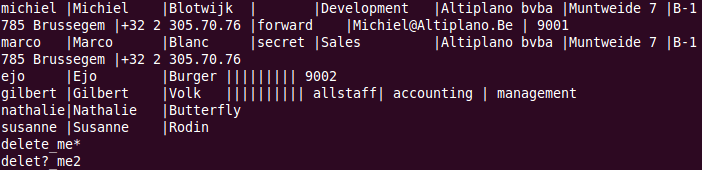
\includegraphics[width=\textwidth]{lat/us00-archivoDeEjemplo.png}
    \caption{Ejemplos de creación y borrado de usuarios}
\end{figure}

Las líneas primera y segunda en realidad serían una única, pero se corta. Lo mismo pasa con las líneas tercera y cuarta. Las dos últimas sólo son válidas para el borrado de usuarios.\\

Si queremos crear una lista completa de usuarios como por ejemplo los que usamos en clase, desde alu01 hasta alu40, tenemos varias alternativas. La primera sería escribir un script que los vaya creando uno a uno usando \lstinline!lat-users -a!:

\begin{lstlisting}
#!/bin/bash

for I in $(seq -w 1 1 40)
do
    lat-users -a -c "alu$I|Alumno|$I|alu$I| | | | | | | | |asir2d"
done
\end{lstlisting}

Los grupos alu01, ..., alu40 se crean automáticamente y se asignan como grupo primario de los correspondientes usuarios.\\

Otra opción es hacer un shell script que escriba un archivo como el users.list que hemos visto anteriormente, y usar luego \lstinline!lat-users -a -i ./users.list!:

\begin{lstlisting}
#!/bin/bash

for I in $(seq -w 1 1 40)
do
    echo "alu$I|Alumno|$I|alu$I| | | | | | | | |asir2d" >> ./users.list  
done
\end{lstlisting}

Puede ocurrir que hayamos escrito el comando erróneamente y se haya creado un usuario o un grupo 'a medias', de manera que no existirá como tal pero seguirá estando en la base de datos, con lo cual no podremos crearlo otra vez. Para eliminar completamente un usuario o grupo en estos casos usaremos:

\begin{lstlisting}
signal-event user-delete usuario
db accounts delete usuario
\end{lstlisting}

O bien

\begin{lstlisting}
signal-event group-delete grupo
db accounts delete grupo
\end{lstlisting}

Un script que viene bien para borrar completamente todos los usuarios añadidos en el ejemplo:

\begin{lstlisting}
#!/bin/bash

lat-users -d -f -c "alu*"

for I in $(seq -w 1 1 40)
do
    signal-event user-delete alu$I
    db accounts delete alu$I
done

signal-event reboot
\end{lstlisting}
